\chapter{Proces tvorby uživatelského rozhraní}
\label{chap:process}

\begin{quote}
\uv{Proces tvorby uživatelského rozhraní je zdokumentovaný postup, který je nutné absolvovat pro dokončení typického uživatelského rozhraní.}
\end{quote}

\noindent
Vývoj každého systému prochází několika fázemi, které se většinou překrývají z důvodu spolupráce vývojářů, designérů a analytiků. Tyto fáze lze rozdělit na čtyři části.

\begin{enumerate}[leftmargin=1cm]
    \item \textbf{Plánování}\\
          Zahrnuje analýzu požadavků klienta a cílové skupiny uživatelů. Dále tato fáze zahrnuje výběr programovacího jazyka, knihoven a dalších nástrojů, které budou použity pro implementaci.

    \item \textbf{Design}\\
          Informace shromážděné z předchozího stádia jsou sepsány a analyzovány. Návrh zahrnuje vývoj struktury a vizuální podoby aplikace a je obvykle rozdělen do tří částí---vytvoření drátěného modelu (anglicky \textit{Wireframe}), grafického návrhu a kódování šablon. Tyto kroky mají za úkol podrobněji specifikovat požadavky klienta a odhalit nejasnosti v zadání. Návrh probíhá převážně paralelně s vývojem.

    \item \textbf{Vývoj}\\
          V této fázi jsou požadované funkce systému implementovány za použití ustanovených technologií a knihoven. Vývoj zahrnuje verifikaci požadavků, integraci grafických návrhů do systému a testování celého systému včetně použitelnosti.

    \item \textbf{Spuštění}\\
           Jedná se o poslední fázi, která prochází nejdelším cyklem. Aplikace je nasazena na produkci. Tento krok je důležitý jednak z důvodů nepředvídatelného chování aplikace na serveru, především však z důvodu hlubšího testování koncovými uživateli.

\end{enumerate}

Tvorba uživatelského rozhraní je provázána se všemi těmito fázemi a zahrnuje několik aktivit, které vyžadují práci s různými nástroji a technologiemi. Tyto aktivity vyžadují rozdílné znalosti a jsou často rozděleny mezi specificky zaměřené specialisty.

\section{Tvorba drátěného modelu}
\label{sec:wireframing}

Webový drátěný model (anglicky \textit{wireframe}) je zjednodušená kresba, která reprezentuje rozmístění prvků a komponent webové stránky; prezentuje strukturální úroveň. Tvorba drátěného modelu zaujímá místo již na začátku životního cyklu projektu a slouží pro zachycení základní struktury stránky. Úkol drátěného modelu je poskytnout vizuální porozumění stránky již na počátku tvorby uživatelského rozhraní.

\begin{figure}[htbp]
    \centering
    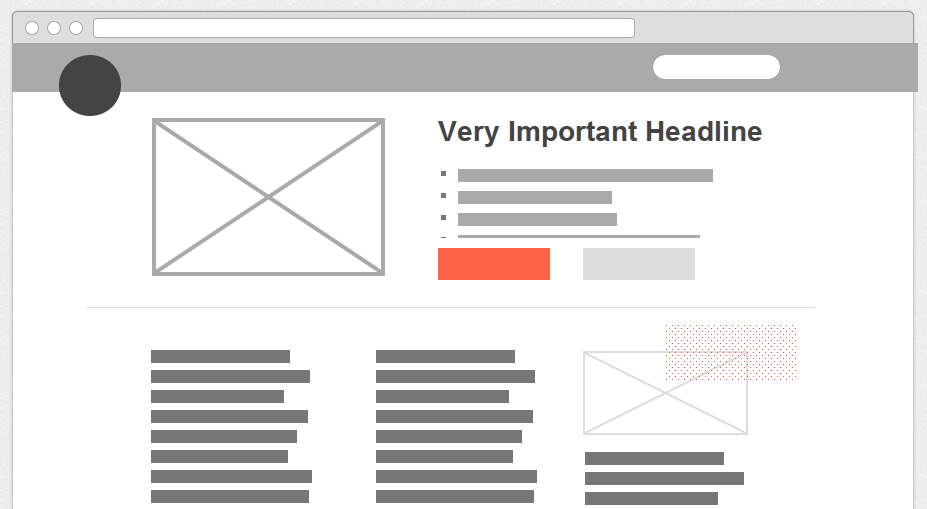
\includegraphics[width=11cm]{images/wireframe-example.png}
    \caption{Příklad drátěného modelu (TODO: zdroj -- wireframe.cc).}
\end{figure}

Výhodou drátěných modelů je jednoduchá přizpůsobitelnost potřebám klienta a jasně definovaná kostra, která zajišťuje sebedůvěru designera. V pozdějších fázích projektu by se neměl drátěný model nijak měnit a měl by odpovídat grafickému návrhu.

\section{Tvorba grafického návrhu}
\label{sec:designing}

Grafický návrh poskytuje vizuální podobu webové aplikace; reprezentuje aplikaci v podobě, ve které bude prezentována uživateli. Tato fáze zahrnuje výběr grafických a typografických prvků. Mezi grafické prvky obyčejně patří kombinace barev, obrázků, tvar tlačítek apod. Typografické prvky zahrnují především organizaci písma -- volbu řezů a rodin písma pro odlišení jednotlivých částí webové stránky. Dále zahrnují velikosti odstavců, odrážky, řádkování atd.

\section{Kódování}
\label{sec:coding}

V tomto stádiu přichází na řadu rozřezání a kódování grafického návrhu. Kódování probíhá v HTML (HyperText Markup Language) a CSS (Cascading Style Sheets). Kód by měl být psán s ohledem na W3C standard (World Wide Web Consortium) a měl by dodržovat osvědčené postupy pro zvýšení čitelnosti a podpory všech nejpoužívanějších prohlížečů.
